\chapter{Results}
\label{ch:results}

%A concept will be developed on how a model for predicting user intent could be built and how it could be applied to the user session.
%To this end, possibilities for collecting and vectorizing sequential UI trees will be discussed
%which are designed to predict the user intent. Here, privacy and feature pre-filteringin UI data plays an important role
%
%After that, personalized as well as collaborative data can be used in a hybrid approach.
%This modelshould then be made available to the user in an Android app service and, depending on the level ofdetail, suggest upcoming apps or actions to the user at a suitable time

This chapter will explain how a prediction model for user intent can be designed and what factors of influence have to be considered.
The design will be shown on the basis of a proof of concept implementation.
Also, a concept of how this model can be applied to the real world is proposed. \todo{check if that is actually done.}

As noted in the introduction the term \ti{intent} has a very wide scope.
It's prediction can only be made in fractions, or serve as indicator.
The semantically closest way and also the most detailed would be to describe the users intent in words, thus a description of what the user wants to do next.
Unfortunately, the users intent description cannot be determined yet, as no according dataset is provided.
An important step, the screen summarization as shown in Screen2words~\ref{subsec:screen2words} \cite{wang2021screen2words}, already was made, which could also be fed with the users intention descriptions.
But this would then only reflect the already passed fulfilled intent and not the upcoming next purpose.
Also, the users flows can be predicted as shown in the works of ERICA~\ref{subsec:erica}.
\todo{may more describe what a 'flow' can do}
Next app prediction already works quite well~\ref{katsarou2022whatsnextapp}, which also reflects the larger intent of the user, but is not very detailed.
In the process of the working on this topic, surprisingly a successful attempt was made to predict the next user interaction, which is explained in section \ref{subsec:user-click-behaviors-deep-learning} \cite{zhou2021large}.
This shows, that it is possible to predict certain user actions upfront.

In order to approximate to reflect the user intent the assumption is made that the next \tb{user interaction} also give hints on what the user is intending to achieve.
The interaction is resulting in another screen, which then the user (hopefully) intends to see.

\todo{Mathematically formulate the problem?}

To provide a basis for further development on this topic, the following criteria were determined.
\begin{itemize}
  \item Make the model as independent of the data as possible (generalization).
  \item Make it extensible for solving other problems, e.g.\ run it as form a classification or apply reinforcement.
  \item Make it accessible to other developers.
  \item Make it reproducible by providing the correct sources and add documentation.
\end{itemize}

\todo{formulate or remove}
Proof of concept, as an example gesture or click traces were used as labels.
%Steps:
%- Data acquisition
%- Data cleaning / Preprocessing (Panadas)
%- Split into Training Data, Validation data, and Test data (cannot adapt the model after using the test data)
%- Train the model with the train data
%- Evaluate the model with the test data, then can adapt the model by the developer
%- Last deploy the model to production

\section{Datasets}

The most relevant datasets already were presented in section~\ref{sec:datasets-of-ui-trees}.
During research a few problems arose, which made it difficult to obtain a dataset which serves the needs of intent prediction.
Most suited datasets, referenced in the papers (by Google and Samsung), were not publicly available.
A promising candidate is the Rico dataset (section~\ref{subsec:rico}), as it provides a huge amount of traces, which is needed for successfully learning a \gls{nn}.
It is also quite up-to-date, which reflects current development and trends.
Trade-offs had to be made in the correctness of the data.
Some samples are missing or don't match with the screenshot.

To overcome these limitations, it is proposed to create a custom dataset, which takes advantage of the accessibility services (section \ref{subsec:android-accessibility-service}).
Traces then can be recorded during transitions of apps (cross-app) or while interacting with the \gls{os}.
The length of a trace would then be extended to a session, defined from activating the screen until it is turned off (by the user or the system itself).
Tracing with accessibility services also has the benefit, that the model could be used locally on the device without communicating with an external provider.
Additional communication and storage of data on servers increases the risk of attacks and leakage, which should be avoided by any circumstances.
On-device processing also is possibly faster, works without internet connection, and makes the application more trustworthy.
A local working technology also facilitate reinforcement learning (section \ref{subsec:machine-learning-types}), which improves the user experience significantly.
Additional features then could also be considered, like sensor data, such as \gls{gps} and gyroscope, acceleration, temperature, light and many more.
A user working with web applications or playing directly rendered games still is a challenge to track, as the accessibility service does not have access to these elements in the same way as for native apps.

% TAKEAWAY: Create custom dataset

\section{Preprocessing Android UI Tree Data}

The widely used dataset Rico was chosen as basis to feed the model.
As noted in section \ref{subsec:rico}, the structure is disaggregated in \ti{app}s, containing \ti{traces}, containing \ti{view hierarchies}, containing \ti{view}s.
A significant aspect is, that the samples in the traces don't get mixed up with other samples, to keep the temporal dependence.
The dataset already was analyzed and manipulated by other researchers, though some of the steps were adopted from Screen2words (section \ref{subsec:screen2words}).
This implicates the feature extraction from the nodes, the bounding box normalization, and the node flattening process (cf. section \ref{subsec:preprocessing}).
The attributes of the Rico dataset (table \ref{tab:rico_view_hierarchy_attributes}) not exactly matching the accessibility tree (cf. listing \ref{android_accessibility_node}), but they are similar enough to state that the process is applicable for both variants.

For the proof of concept these attributes were extracted: \code{bounds} (inherits four values), \code{visibility}, \code{clickable} and the \code{class}.
Also, the nodes depth in the dom tree was calculated, apparent as \code{obj_dom_pos} and the visibility for the user was validated with \code{visibility_to_user_seq}.
One screen exists of multiple views / components, which all have their own attributes.
To be able to examine each screen as one sample, the view hierarchy had to be flattened.
This was done by separating the views by attributes and merge each value by its feature.
Therefore, a screen sample was converted to a list of features, which again holds a list of values.
This is an important step to realize as the dataset now consists of four array dimensions, which plays a big role in later steps, as it makes further processing more challenging.
The gesture traces were acquired from the dataset to provide them as labels, but also as additional input.
They contain one (click) or multiple (swipe) coordinates.
For simplification only the first value was considered, but it is proposed to also provide the other values as input.
Then all traces were iterated through and samples were filtered out, which did not provide any features.
Also, only traces were picked, which did provide six or more screen samples, to be able to train a sequential model, resulting in 4278 traces with 50301 samples.
Then the features consisting of arrays were padded to the same length (here: 500).
This could be done per feature, but it was uniquely applied, because the number of views and therefore the length for each nested feature array is the same.

The data then was split in a train and a validation set.
Due to the limiting capacity of the \gls{gpu}, only 20\% of the traces were used.
Therefore, 642 traces were selected for training and 213 for validation.
The following processing applied equally, but executed separately for train and test split.

The input and output (label) pairs were generated, which had to be done after splitting the traces to keep the temporal order.
Therefore, for each trace the first samples $s$ (here: 5) acted as the input sequence $I$ and the next one (here: sixth) was the label $L$ (cf.\ figure~\ref{fig:model-structure}).
This step was repeated by shifting the samples by one, so that the first sample was dropped and the label from the previous record then was part of the second input sequence.
As label then served the next (here: seventh) sample.
This process was done until no sample was left in the trace, that could take the role of the label.
For the case of the proof-of-concept all features were dropped from the labels, except the click / gesture position values $f_1$ and $f_2$, because that's the prediction that has been looked for.
After the input and output pairs for each trace have been generated, they then could be finally merged together in one array.
The reason is that the input sequences and labels were then fixed and didn't depend on the upcoming samples in the trace.

\subsection{Filtering privacy invasive details}

\todo{todo}
- rico doesn't use logins or any privat data
- gestures can tell more about the user
-

\section{Model}

In the proof-of-concept a very dynamic approach was selected to be able to support new features without major changes.
Therefore, depending on the input features $f$, the model was adapted automatically by these rules (cf.\ figure~\ref{fig:model-structure}):

\begin{itemize}
  \item If the sample feature consisted of a single value, it was directly passed for further processing.
  \item If the sample feature included multiple values, they were reduced in the dimensionality (dense layer) based on the length and provided each output value as a separate feature dimension.
  \item If the sample feature provided a continuous numerical value (normalized), it was also directly passed to be processed further.
  \item If the sample feature provided a categorical value (indexed), it was embedded (section \ref{subsec:embedding-layer}) and then flattened to match the array dimensionality.
\end{itemize}

% https://stackoverflow.com/questions/54743549/is-it-possible-to-making-lstm-model-with-4-dimension-shape-of-data
For simplicity all categorical values were handed over as array as it would not make a difference in processing.
The numerical and categorical embeddings then were concatenated together and handed over to the \gls{lstm}.
The \gls{lstm} expects an array / space dimension of three.
The first array dimension is the sample dimension (unlimited), which in this case is the list of all sample sequences.
The second array dimension is the time step dimension (fixed size), thus the sample sequence itself.
The third array dimension is the feature dimension (fixed size), therefore there's no dimension left to encode nested or even variable arrays, such as multiple views / components.
For that reason multiple embedded category values had to be flattened (reshaped) before entering the \gls{lstm} model with 128 neurons.

\todo{link and explain LSTM (?)}
%TimeDistributedLayer
% https://stackoverflow.com/a/61588937/5164462
% https://stackoverflow.com/questions/53107126/what-are-the-uses-of-timedistributed-wrapper-for-lstm-or-any-other-layers

The output of the \gls{lstm} then was passed to a dense layer with 32 neurons, followed by a dropout of 20\% of neurons.
Finally, the values were passed to the output layer with two neurons, which were representing the $x$ (Gest$_x$) and $y$ (Gest$_y$) axis of the predicted gesture.

Due to all the numerical and categorical features chosen from the dataset, the model \tb{SelectedFeatures} in figure~\ref{fig:model-structure} crystallized.

\todo{typo in figure: "continuous"}
\begin{figure}[htbp!]
  \centering
  \makebox[\textwidth][c]{\includesvg[width=1.2\textwidth]{graphics/model_structure.svg}}
  \caption[Structure of user intent prediction model]{Structure of the proposed intent prediction model, $I_k$ is the $k$th input sequence, $L_k$ is the $k$th label from the sequence, $s_m$ is the $m$th sample in the sequence, $f_n$ is the $n$th feature of a sample.}
  \label{fig:model-structure}
\end{figure}

The above structure also allows to take in more features as prediction.
Then it has to be reconsidered, at to which screen the gesture or click belongs to.
Is it wanted to predict the next screen from the current screen and its gestures?
Or is it desired to predict the gestures made by the user on the current screen and also predict the views of the next screen?

While the design process of the model, multiple approaches were considered.

One procedure would be to use a pretrained embedding for Android UIs, e.g. the Screen2vec embedding of \cite{li2021screen2vec} in section \ref{subsec:screen2vec}.
The big advantage is, that the screens are already reduced to a vector and the \gls{rnn}, like the \gls{lstm}, has much more valuable inputs and therefore requires less time for training.
This also comes with a disadvantage: the backpropagation process cannot be applied to the pretrained model and the features which are important for training a temporal dependent model may differ from the needed features e.g. similarity of screens based on an \gls{ae}.

More approaches have to be considered, when not just want to predict the click position, but rather a view element or even the whole screen should be forecasted.
Then due to the high dimensionality of the output, it could make sense to precede an \gls{ae} net before the \gls{rnn} layer, to work out important features.
This would have a similar structure as the pretrained embedding, but is adaptable during training.
The decoder of the \gls{ae} then also can be moved to after the \gls{rnn} layer, which should improve the performance.
Or the encoder and the decoder are subsequently processed afterwards to provide all raw feature inputs to the \gls{rnn}.

As earlier mentioned, an even more promising approach, which has been proved to work well in click sequence prediction (section \ref{subsec:user-click-behaviors-deep-learning}), is the transformer (section \ref{subsubsec:transformer}).

\section{Evaluation}

To get an insight of what features are providing valuable information, a second model was built, which only included the click / gesture sequence as feature, referenced as \tb{ClickOnly}.
During preparing the dataset an important step was missing, which could help improving performing better.
Only the click of the next screen was predicted, but not the click on the current screen.
Therefore, all click values were shifted by one step and filled up with a value of $0.5$ which represents the mid of the screen.
The idea is that the click now belongs to the screen which is shown after the action.
In theory that should improve the models performance, as it then can choose the click based on the elements shown on the current screen while predicting.
This experiment is referenced as \tb{FeaturesClickShifted}.

In the figures of \ref{fig:model_history_losses} the training loss and the validation loss can be seen for all three approaches.
A numbered representation of the last epoch for each model is listed in the table \ref{tab:model_losses}.
The models all were trained with the \gls{adam} optimizer by using the \gls{mse} as loss metric.

In all three models, the loss was around 0.09 for the validation set.
This is a deviation of 0.3 for the \gls{rmse}.
That means for a screen from left \tb{0} to right \tb{1} and bottom \tb{0} to top \tb{1}, the predicted point (click) was around $0.3$ away projected to the euclidean distance.
To put it in perspective, if the center is used as prediction, it is off by a maximum of $0.5$, if the expected user click is always at the border.
But in the mean the clicks are even closer.
To check that the \gls{rmse} was calculated, if all predictions were made to $0.5$ for Gest$_x$ and Gest$_y$, resulting in $0.3102$.
Using the mean for Gest$_x$ ($0.4360$) and Gest$_y$ ($0.4552$) resulted in a \gls{rmse} of $0.3052$.
This implies that the models predicting the user clicks only slightly better than the statistical mean.
In contrast to the expectation, shifting the click sequence in FeaturesClickShifted did not result in much better predictions compared to the SelectedFeatures model, at least not with the small amount of training data.
Even the ClickOnly model performed better, with no additional features.
As buttons are scattered all around the screen, $0.3$ \gls{rmse} seems a reasonable value, if the models always predicts the mean as the next click interaction.

Regarding the number of epochs, the ClickOnly model needed less than the others, which is expected as it has only two feature dimensions.
The other two models needed more epochs to align with the values of the ClickOnly model.
This can be the result of aligning the additional random weights for all the additional features.
The FeaturesClickShifted model needed slightly more epochs than the SelectedFeatures model, which could be by chance, or it found slightly more correlations than the SelectedFeatures model.
%\todo{calculate mean distance from center}
%the \gls{rmse} of 0.3102 with 0.5
%0.3052 with mean
%0.3060 with median
%
%x has median value of 0.4259, mean value of 0.4360
%y has median value of 0.4248, mean value of 0.4552

\begin{figure}[htbp!]
  \centering
  \begin{subfigure}[b]{0.45\textwidth}
    \centering
    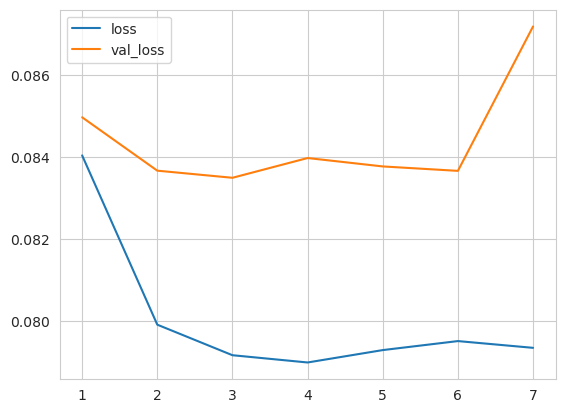
\includegraphics[width=\textwidth]{graphics/model_history_loss_clicks}
    \caption{ClickOnly: Only clicks as features}
    \label{fig:model_history_loss_clicks}
  \end{subfigure}
  \hfill
  \begin{subfigure}[b]{0.45\textwidth}
    \centering
    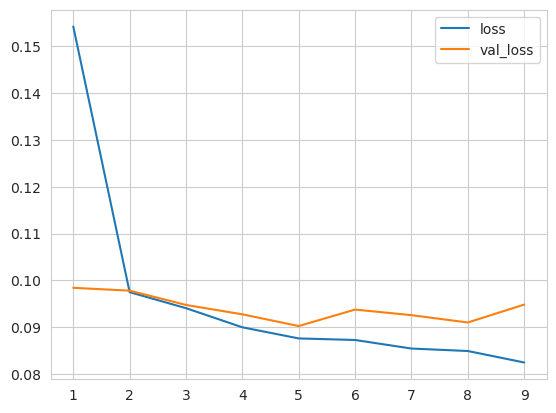
\includegraphics[width=\textwidth]{graphics/model_history_loss_features}
    \caption{SelectedFeatures: Bounding box and click features}
    \label{fig:model_history_loss_features}
  \end{subfigure}
  \hfill
  \begin{subfigure}[b]{0.8\textwidth}
    \centering
    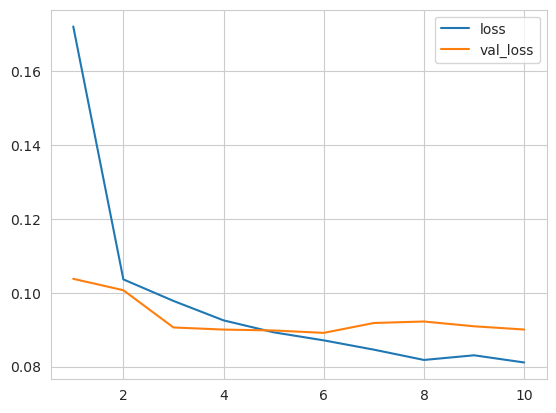
\includegraphics[width=\textwidth]{graphics/model_history_loss_features_shifted}
    \caption{FeaturesClickShifted: Bounding box and shifted click features}
    \label{fig:model_history_loss_features_shifted}
  \end{subfigure}
  \caption[Training loss vs. validation loss]{Training loss (\ti{loss}, blue) vs. validation loss (\ti{val\_loss}, orange). Horizontal axis is the number of epochs. Vertical axis is the loss as \gls{mse}.}
  \label{fig:model_history_losses}
\end{figure}

\begin{table}[htbp!]
  \small
  \centering
  \begin{tabular}{|l|l|l|l|l|}
    \hline
    \textbf{Method}      & \textbf{Loss} & \textbf{Validation Loss} & \textbf{RMSE Val Loss}   & \textbf{Number of epochs} \\
    \hline
    ClickOnly            & 0.0793        & 0.0872                   & 0.2953                   & 7                         \\
    SelectedFeatures     & 0.0824        & 0.0948                   & 0.3079                   & 9                         \\
    FeaturesClickShifted & 0.0811        & 0.0900                   & 0.3000                   & 10                        \\
    \hline
  \end{tabular}
  \caption[Training and validation loss, number of epochs]{Training and validation loss (\gls{mse}) of all three models, ClickOnly, SelectedFeatures and FeaturesClickShifted}
  \label{tab:model_losses}
\end{table}



